
% Generated from data/datasheet.json. Do not edit this file manually.
\newcommand{\DatasheetVersion}{1.1.1}
\newcommand{\DatasheetVersionLabel}{v1.1.1}
\newcommand{\DatasheetBody}{%
\enlargethispage{18pt}
% --- TITLE HEADER ---
\begin{figure}[h!]
    \begin{minipage}[c]{0.55\textwidth}
        \raggedright
        {\color{brandblue}\Huge \textbf{RPi CM5 Interface Board}} \\[0.2cm]
        {\Large Breakout board for the Raspberry Pi Compute Module 5} \\[0.15cm]
        {\large \textcolor{brandblue}{\textbf{Board Version \DatasheetVersion}}} \\[0.4cm]

        \textbf{\large Features}
        \begin{itemize}[leftmargin=*, nosep]
            \item Safe RPi Shutdown
            \item Status LEDs
            \item Programmable RGB LED
            \item IMU (Bosch BHI260AP)
            \item SD Card Slot
            \item Real-Time Clock
            \item Test Points
        \end{itemize}
    \end{minipage}
    \hfill
    \begin{minipage}[c]{0.4\textwidth}
        \raggedleft
        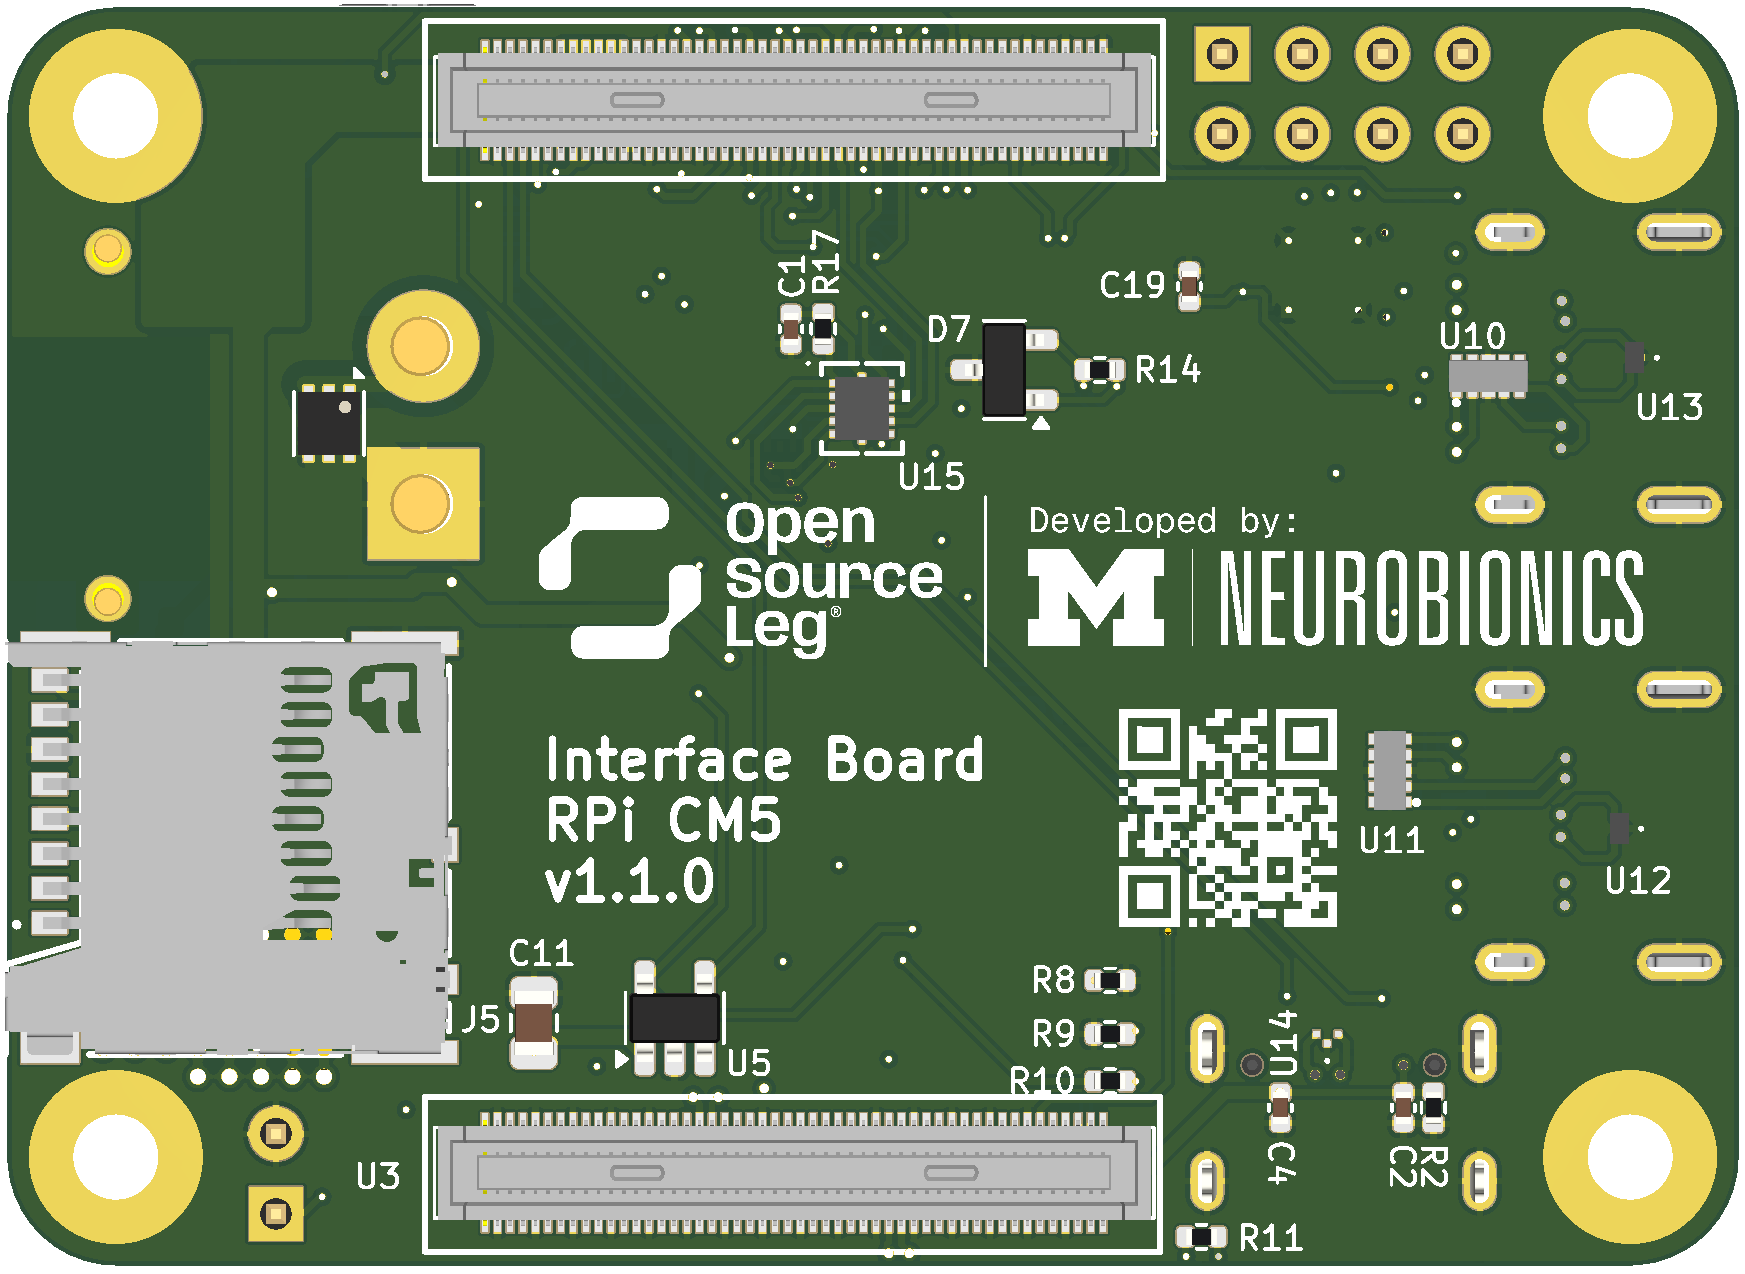
\includegraphics[width=0.95\textwidth]{pcb-front.png}
    \end{minipage}
\end{figure}

% --- OVERVIEW ---
\section{Overview}
The RPi CM5 Interface Board is an add-on module for the Raspberry Pi Compute Module 5 (RPi CM5) that is designed to provide plug and play functionality for sensors and actuators across a wide variety of robotics applications. It is built and tested by researchers at the University of Michigan's Neurobionics Lab.

% --- TECHNICAL SPECS ---
\section{Technical Specifications}
\begin{table}[h!]
    \centering
    \renewcommand{\arraystretch}{1.3}
    \begin{tabularx}{\textwidth}{l X}
    \toprule
    \textbf{Category} & \textbf{Specification} \\
    \midrule
    \textbf{Input Voltage} & 15V -- 48V (XT30) | 5V (USB-C) \\
    \textbf{Power Output} & 5V @ 5A (SMPS) | 3.3V @ 1A (LDO) \\
    \textbf{Module Support} & Raspberry Pi Compute Module 5 (CM5) / CM5 Lite \\
    \textbf{USB Interface} & 2x USB-C 3.0 (High-Speed Communication) \\
    \textbf{CAN Bus} & 2x CAN Bus (MCP2515 Controller + MCP2562 Transceiver) \\
    \textbf{Sensors} & Bosch BHI260AP (6-Axis IMU) on SPI0 chip select 1 \\
    \textbf{Storage} & MicroSD Card Slot (for CM5 Lite boot/storage) \\
    \textbf{Cooling} & 4-Pin Fan Connector (PWM Control + Tachometer) \\
    \textbf{Dimensions} & 55.00 mm x 40.00 mm x 14.09 mm \\
    \bottomrule
    \end{tabularx}
\end{table}

% --- PINOUTS ---
\section{Pinout \& Interfaces}
\begin{minipage}[t]{0.48\textwidth}

    \subsection*{UART-1 (Molex PicoClasp, 4-Pin)}
    \begin{minipage}[t]{0.60\textwidth}
        \begin{tabularx}{\textwidth}{c X}
        \toprule
        \textbf{Pin} & \textbf{Function} \\
        \midrule
        1 & +3.3V \\
        2 & UART1\_TX \\
        3 & UART1\_RX \\
        4 & GND \\
        \bottomrule
        \end{tabularx}
    \end{minipage}%
    \hfill
    \begin{minipage}[t]{0.35\textwidth}
        \centering
        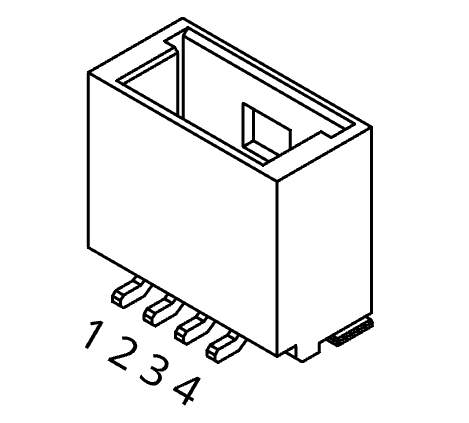
\includegraphics[width=\linewidth]{4pin_pico.png}
    \end{minipage}

    \vspace{0.6cm}

    \subsection*{UART-2 (Molex PicoClasp, 4-Pin)}
    \begin{minipage}[t]{0.60\textwidth}
        \begin{tabularx}{\textwidth}{c X}
        \toprule
        \textbf{Pin} & \textbf{Function} \\
        \midrule
        1 & +3.3V \\
        2 & UART2\_TX \\
        3 & UART2\_RX \\
        4 & GND \\
        \bottomrule
        \end{tabularx}
    \end{minipage}%
    \hfill
    \begin{minipage}[t]{0.35\textwidth}
        \centering
        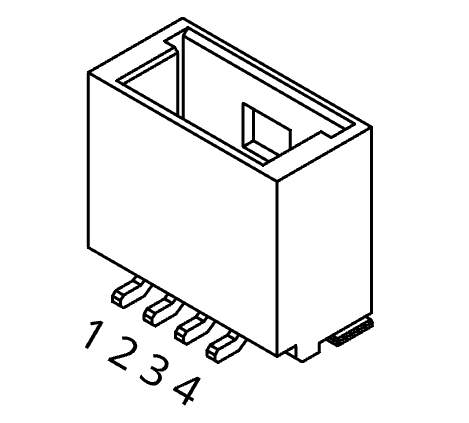
\includegraphics[width=\linewidth]{4pin_pico.png}
    \end{minipage}

    \vspace{0.6cm}

    \subsection*{I2C-2 (Molex PicoClasp, 4-Pin)}
    \begin{minipage}[t]{0.60\textwidth}
        \begin{tabularx}{\textwidth}{c X}
        \toprule
        \textbf{Pin} & \textbf{Function} \\
        \midrule
        1 & +3.3V \\
        2 & I2C2\_SDA \\
        3 & I2C2\_SCL \\
        4 & GND \\
        \bottomrule
        \end{tabularx}
    \end{minipage}%
    \hfill
    \begin{minipage}[t]{0.35\textwidth}
        \centering
        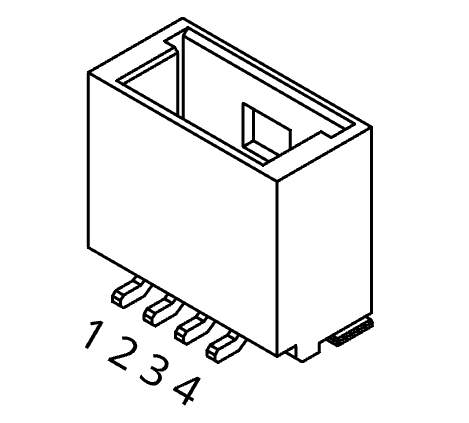
\includegraphics[width=\linewidth]{4pin_pico.png}
    \end{minipage}

    \vspace{0.6cm}

    \subsection*{I2C-3 (Molex PicoClasp, 4-Pin)}
    \begin{minipage}[t]{0.60\textwidth}
        \begin{tabularx}{\textwidth}{c X}
        \toprule
        \textbf{Pin} & \textbf{Function} \\
        \midrule
        1 & +3.3V \\
        2 & I2C3\_SDA \\
        3 & I2C3\_SCL \\
        4 & GND \\
        \bottomrule
        \end{tabularx}
    \end{minipage}%
    \hfill
    \begin{minipage}[t]{0.35\textwidth}
        \centering
        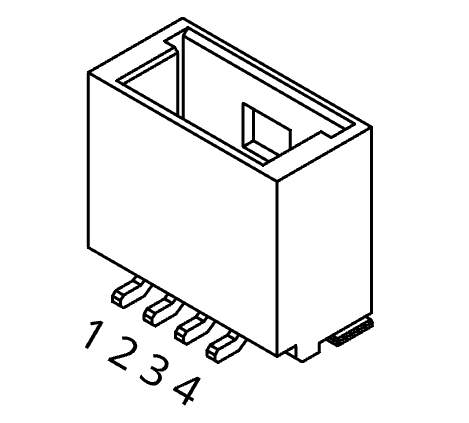
\includegraphics[width=\linewidth]{4pin_pico.png}
    \end{minipage}

    \vspace{0.6cm}
\end{minipage}
\hfill
\begin{minipage}[t]{0.48\textwidth}

    \subsection*{SPI-1 (Molex PicoClasp, 8-Pin)}
    \begin{minipage}[t]{0.60\textwidth}
        \begin{tabularx}{\textwidth}{c X}
        \toprule
        \textbf{Pin} & \textbf{Function} \\
        \midrule
        1 & +3.3V \\
        2 & SPI1\_CSn2 \\
        3 & SPI1\_CSn1 \\
        4 & SPI1\_CSn0 \\
        5 & SPI1\_SCLK \\
        6 & SPI1\_MISO \\
        7 & SPI1\_MOSI \\
        8 & GND \\
        \bottomrule
        \end{tabularx}
    \end{minipage}%
    \hfill
    \begin{minipage}[t]{0.35\textwidth}
        \centering
        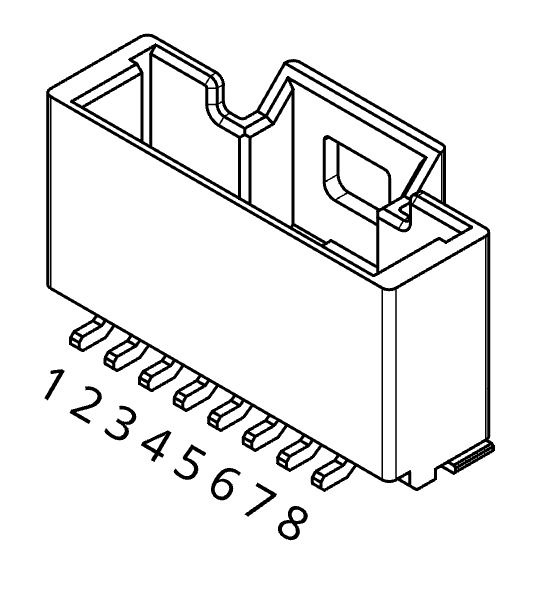
\includegraphics[width=\linewidth]{8pin_pico.png}
    \end{minipage}

    \vspace{0.6cm}

    \subsection*{CAN-0/1 (Molex PicoClasp), 3-Pin)}
    \begin{minipage}[t]{0.60\textwidth}
        \begin{tabularx}{\textwidth}{c X}
        \toprule
        \textbf{Pin} & \textbf{Function} \\
        \midrule
        1 & GND \\
        2 & CAN\_P \\
        3 & CAN\_N \\
        \bottomrule
        \end{tabularx}
    \end{minipage}%
    \hfill
    \begin{minipage}[t]{0.35\textwidth}
        \centering
        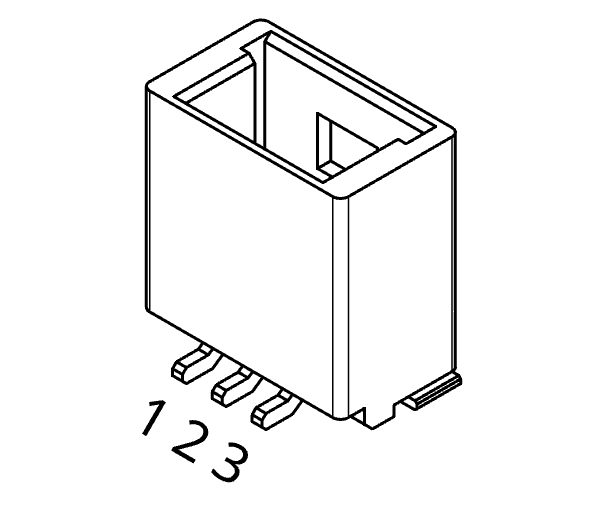
\includegraphics[width=\linewidth]{3pin_pico.png}
    \end{minipage}

    \vspace{0.6cm}

    \subsection*{GPIO HEADERS}
    \begin{minipage}[t]{0.60\textwidth}
        \begin{tabularx}{\textwidth}{c X}
        \toprule
        \textbf{Pin} & \textbf{Function} \\
        \midrule
        1 & GPIO\_25 \\
        2 & GPIO\_23 \\
        3 & GPIO\_7 \\
        4 & +3.3V \\
        5 & GPIO\_27 \\
        6 & GPIO\_24 \\
        7 & GPIO\_22 \\
        8 & GND \\
        \bottomrule
        \end{tabularx}
    \end{minipage}%
    \hfill
    \begin{minipage}[t]{0.35\textwidth}
        \centering
        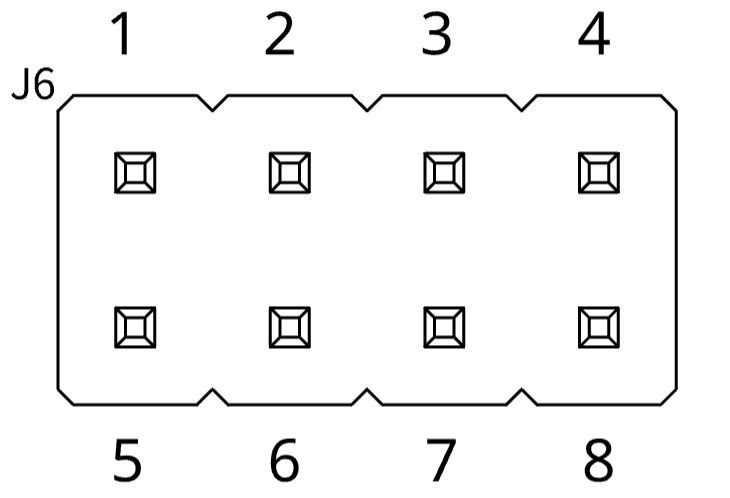
\includegraphics[width=\linewidth]{pinheader_number.png}
    \end{minipage}

    \vspace{0.6cm}

    \subsection*{Fan Port, JST 4-Pin Connector}
    \begin{minipage}[t]{0.60\textwidth}
        \begin{tabularx}{\textwidth}{c X}
        \toprule
        \textbf{Pin} & \textbf{Function} \\
        \midrule
        1 & Tachometer \\
        2 & GND \\
        3 & PWM \\
        4 & +5V \\
        \bottomrule
        \end{tabularx}
    \end{minipage}%
    \hfill
    \begin{minipage}[t]{0.35\textwidth}
        \centering
        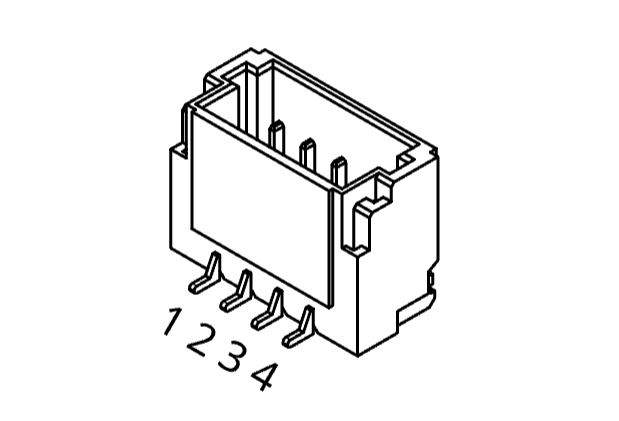
\includegraphics[width=\linewidth]{fanport_numbering.png}
    \end{minipage}

    \vspace{0.6cm}
\end{minipage}

\clearpage
% --- MECHANICAL ---
\section{Mechanical Details}
\begin{itemize}
    \item \textbf{PCB Dimensions:} $55\,\si{mm} \times 40\,\si{mm}$
    \item \textbf{Mounting Holes:} 4 x 2.7 mm (Standard M2.5)
    \item \textbf{Max Height:} $14.09\,\si{mm}$ (Top of USB-C connector to bottom pins)
\end{itemize}

\begin{figure}[h!]
    \centering
    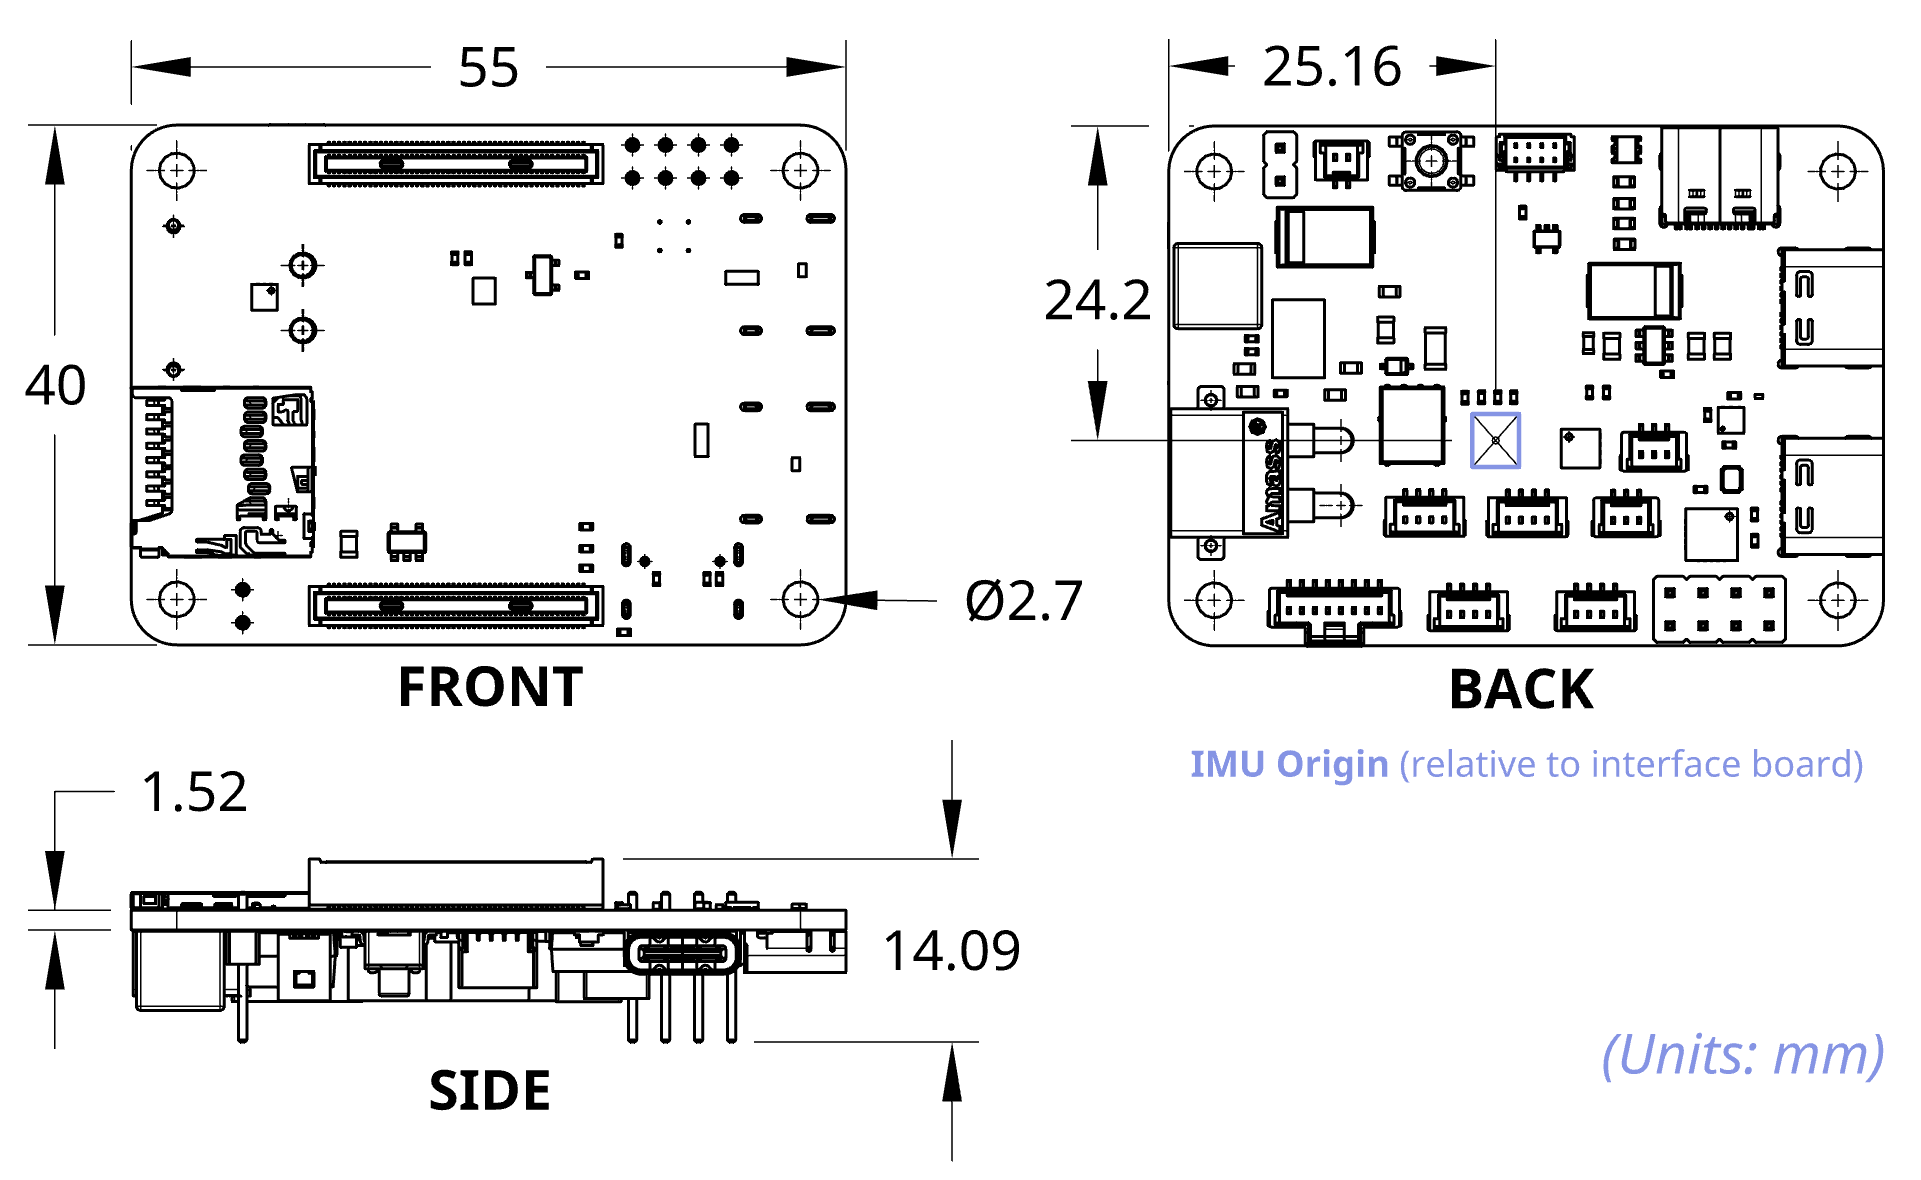
\includegraphics[width=0.9\textwidth]{mechanical_specs.png}
    \caption{Mechanical Drawing \& Sensor Origin}
\end{figure}

% --- OTHER COMPONENTS ---
\section{Other Components}
\begin{itemize}[leftmargin=*]
    \item \textbf{Signal LEDs:} 5V, 3.3V, Power, and Activity
    \item \textbf{Programmable RGB LED:} Addressable RGB LED for user feedback and debugging
    \item \textbf{J4 External Switch:} Can be used for safe RPi shutdown with an external switch using a Molex PicoClasp 2-pin connector
    \item \textbf{Safe Shutdown Circuit:} Allows clean shutdown of the Raspberry Pi without power corruption
    \item \textbf{Real-Time Clock (RTC):} Maintains system time when RPi is off (only interface board is powered).
    \item \textbf{Test Points:} Labeled test points for power rails and key signals to assist debugging
    \item \textbf{Boot Configuration Access:} Hardware support for CM5 boot and bring-up workflows
\end{itemize}

% --- REVISION HISTORY ---
\section{Revision History}

    \subsection*{v1.1.1 -- August 2026}


        \textbf{Changes:}
        \begin{itemize}[leftmargin=*, nosep]
            \item Power supply layout improvements
        \end{itemize}


    \subsection*{v1.1.0 -- May 2026}

        \textbf{New Features:}
        \begin{itemize}[leftmargin=*, nosep]
            \item Added 2nd CAN bus
            \item RGB LED now enabled
            \item RTC pulled up to remain on when Pi is powered off
            \item ESD protection diodes on all USB-C data and power lines
            \item TVS diode for surge current protection on XT30 input
        \end{itemize}

        \textbf{Changes:}
        \begin{itemize}[leftmargin=*, nosep]
            \item Modified I2C port configuration
            \item Modified IMU location on board
        \end{itemize}


    \subsection*{v1.0.0 -- October 2025}

        \textbf{New Features:}
        \begin{itemize}[leftmargin=*, nosep]
            \item Programmable RGB LED port
            \item IMU integration
            \item Multiple SPI chip selects
            \item GPIO pin breakouts
            \item New OSL symbol
        \end{itemize}


        \textbf{Fixes:}
        \begin{itemize}[leftmargin=*, nosep]
            \item Reduced LED brightness
            \item SD card functionality restored
            \item Improved thermal management
            \item Added flipped USB-C support
            \item 3.3V line enable
        \end{itemize}
}
